\documentclass[12pt]{article}

\usepackage[utf8]{inputenc}
\usepackage{amsmath}
\usepackage{graphicx}
\usepackage{titlesec}
\usepackage{tcolorbox}
\usepackage{titling}
\usepackage{circuitikz}
\usepackage{enumitem}
\usepackage{wrapfig}

\title{\bfseries Laborator Electricitate 3}
\author{Sîrghe Matei}
\date{\today}

\pretitle{\begin{center}\LARGE\bfseries}
\posttitle{\par\end{center}\vskip 0.5em}
\preauthor{\begin{center}\large}
\postauthor{\end{center}}
\predate{\begin{center}\large}
\postdate{\end{center}}

\titleformat{\section}
  {\normalfont\Large\bfseries}{\thesection}{1em}{}

\begin{document}

\maketitle

\begin{center}
    \LARGE\textit{Studiul condensatorului electric cu fețe plan-paralele și}
    \LARGE\textit{Determinarea constantei dielectrice a unui izolator}
\end{center}

\section{Teoria Lucrării}

\subsection{Schema Electrică}

\begin{minipage}{0.45\textwidth}
    \centering
    \textbf{Notație condensator :}
    \begin{circuitikz} \draw
        (0,0) to[C] (2,0);
    \end{circuitikz}
\end{minipage}
\hfill
\begin{minipage}{0.45\textwidth}
    \centering
    \begin{circuitikz} \draw
        (0,0) to[ground] (0,-0.2) node[ground] {}
        (0,0) to[battery] (2,0)
        to[C] (4,0)
        to[ground] (5,0) node[ground] {};
        \draw (2,1) node[right] {$+Q$};
        \draw (3,1) node[right] {$-Q$};
        \draw (2,-1) node[right] {$5C$};
        \draw (3,-1) node[right] {$-5C$};
    \end{circuitikz}
\end{minipage}


\noindent
\textbf{Definiție : }Condensatorul electric este un dispozitiv format din doua plăci metalice așezate față în față separate de un mediu izolator sau dielectric.
Plăcile metalice ale condensatorului se numesc armături și se încarcă cu aceeași cantitate de sarcină electrică dar de semn opus. Proprietatea
fundamentală a unui condensator electric este aceea de a înmagazina $($reține$)$ pentru un anumit interval de timp sarcină electrică.

\noindent
\textbf{Mărimi fizice :} $[C]_{SI}$ Mărimea fizică care descrie comportamentele unui condensator electric se numește
capacitate electrică și în sistemul internațional de unități se măsoară în \textbf{Farad}.

\begin{center}
    \centering
    \begin{circuitikz} \draw
        (0,0) to[ground] (0,-0.2) node[ground] {}
        (0,0) to[battery] (2,0)
        to[C] (4,0)
        to[ground] (5,0) node[ground] {};
        \draw (2,1) node[right] {$+Q$};
        \draw (3,1) node[right] {$-Q$};
        \draw (2,-1) node[right] {$\rho_{N}$};
        \draw (3,-1) node[right] {$\rho_{M}=0$};
    \end{circuitikz}
\end{center}

\noindent
\textbf{Formule fizice :}
\begin{enumerate}
    \item $[C]_{SI}$ = 1 F (Farad) = 1 C/V (Coulomb pe Volt)
    \item $C=\frac{+Q}{\rho_{N}-\rho_{M}}=\frac{-Q}{\rho_{M}-\rho_{N}}=\frac{\left| Q \right|}{U_{NM}}$
    \item $\Delta\rho = U $ - tensiune electrică
    \item $\left| \rho_{M}-\rho_{N} \right| = U_{NM} $ - Diferența de potențial 
\end{enumerate}

\subsection{Montajul Experimental}

\begin{center}
    \centering
    \begin{circuitikz} \draw
        (0,0) to[ground] (0,-2) node[ground] {}
        (0,0) to[battery] (2,0)
        to[C] (5,0)
        (5,0)to[ground] (5,-2) node[ground] {}
        (5,0) to[C] (6,0)
        
        (8,0) node[op amp] (opamp) {};
        \draw (opamp.+) -- ++(0,-0.5) -| (5,0) {};
        \draw (opamp.-) -- ++(0,0) -| (6,0);
        \draw (opamp.out)(9,0) to[voltmeter] (10,0) node[right] {Out};

        \draw (0,-1) node[right] {$[\rho]=V$};
        \draw (0,1) node[right] {$+$};
        \draw (2.5,0.5) node[right] {$+Q$};
        \draw (3.5,0.5) node[right] {$-Q$};
        \draw (3.25,-0.75) node[right] {$C$};
        \draw (5.25,-0.75) node[right] {$C_{0}$};
    \end{circuitikz}
\end{center}

\subsection{Determinarea capacității electrice necunoscute C}
Valoarea lui C va fi determinată prin metoda grafică.\\

$C=\frac{Q}{\rho}$ \hspace{2cm} $C_{0}=\frac{Q}{U}$ \hspace{2cm}  $Q=C_{0}U \hspace{2cm}  C=\frac{C_{0}*U}{\rho}$\\

$\rho- $ Este modificat \hspace{2cm} $U- $Date primare\\

\begin{tcolorbox}[colback=yellow!10!white, colframe=black, title=Observație]
Teoria discutată la acest punct al experimentului este validă dacă și numai dată distanța dintre cele două armături (d) este constantă.
\end{tcolorbox}

\subsection{Verificarea legii C \textasciitilde $\frac{1}{d}$}
Distanța dintre armături va fi modificată astfel încât să putem verifica legea C \textasciitilde $\frac{1}{d}$.\\

$C=\frac{Q}{\rho}$ \hspace{2cm} $C_{0}=\frac{Q}{U}$ \hspace{2cm}  $Q=C_{0}U \hspace{2cm}  C=\frac{C_{0}*U}{\rho}$\\

$d- $ Este modificat \hspace{2cm} $C- $Calculat de noi\\

\begin{tcolorbox}[colback=yellow!10!white, colframe=black, title=Observație]
Teoria discutată pentru acest subpunct al experimentului este validă dacă și numai dacp diferența de potențial aplicată cu ajutorul
sursei de înaltă tensiune rămâne constantă. ($\rho- $ cnst.)
\end{tcolorbox}

\subsection{ Determinarea constantei dielectrice a unui izolator \textbf{$(\epsilon_{r})$}}

\begin{wrapfigure}{r}{0.5\textwidth} 
    \centering
    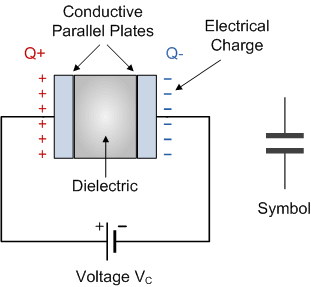
\includegraphics[width=0.38\textwidth]{dielectric.png} 
    \caption{Izolator dielectric}
    \label{fig:Dielectric}
\end{wrapfigure}

Pentru punctele a) și b) izolatorul considerat a fost aer. Pentru acest punct, vom face mai întâi determinări experimentale folosind aerul
ca izolator iar apoi în același condiții experimentale vom face măsurători folosind o placă de plastic pe care o vom introduce între cele două armături.

$\rho$ = constant ; d=constant \\

$C_{aer}=\frac{Q_{aer}}{\rho_{aer}}$  ;  $C_{0}=\frac{Q_{aer}}{U_{aer}}$\\

$C_{aer}=\frac{C_{0}*U_{aer}}{\rho}$  ; $\rho_{aer}=\rho$\\

$C_{izolator}=\frac{Q_{izolator}}{\rho}=\frac{C_{0}*U_{izolator}}{\rho}$\\

$\epsilon_{r}=\frac{C_{izolator}}{C_{aer}}$  ;  $\epsilon_{r}-adimensional$\\



\section{Datele Experimentului Primare}
Datele experimentale primare reprezintă datele culese din laborator în timpul efectuării lucrării de laborator și trebuie scrise complet așa
cum sunt citite de pe aparatele de măsură. Mărimea fizică citită va fi însoțită de unitatea de măsură aferentă.


\section{Prelucrarea datelor experimentale}
Această secțiune reprezintă aportul avut de fiecare în realizarea referatului de laborator. Dacă datele experimentale primare nu sunt exprimate
în unități ale sistemului internațional de unități, atunci se va face conversia.

Graficele se vor insera la lucrarea de laborator căreia îi aparțin și nu la finalul tuturor lucrărilor de laborator. Graficele se vor face fie folosind
un program specializat, fie pe hârtie milimetrică. Curbele Graficului se vor trasa cu creionul.


Numărul zecimalelor indicate în urma calculelor matematice trebuie corelate cu numărul zecimalelor citite în laborator.


\section{Concluzii}
Concluzia referatului trebuie să fie scurtă,(1-2 propoziții) și să indice principalul rezultat obținut după efectuarea lucrării de laborator.


\end{document}